
\section{Casos de uso}

\subsection*{Encargado de compras}
\begin{enumerate}
	\item Consultar precios disponibles para un producto, 
	por número de parte, 
	para optar por el proveedor que ofrece mejores condiciones.
	\item Conocer los precios de la competencia,
	para descubrir oportunidades.
	\item Seguir el stock disponible,
	previendo necesidades de corto y mediano plazo.
\end{enumerate}

\subsection*{Encargado de ventas}
\begin{enumerate}
	\item Conocer los precios de la competencia.
	\item Conocer precio promedio de recompra.
	\item Conocer el margen actual para un producto,
	para fijar precios que permitan encontrar un equilibrio entre competitividad y margen de ganancia,
	así como fidelizar a los mejores clientes.
\end{enumerate}

\subsection*{Personal de ventas}
\begin{enumerate}
	\item Consultar precios de los productos para informar al consumidor final.
	\item Emitir factura electrónica,
	autorizada por ARCA.
\end{enumerate}

\section{Diagrama de casos de uso}

\begin{figure}[ht]
	\vspace{20pt}
	\centering
	\vspace{15pt}
	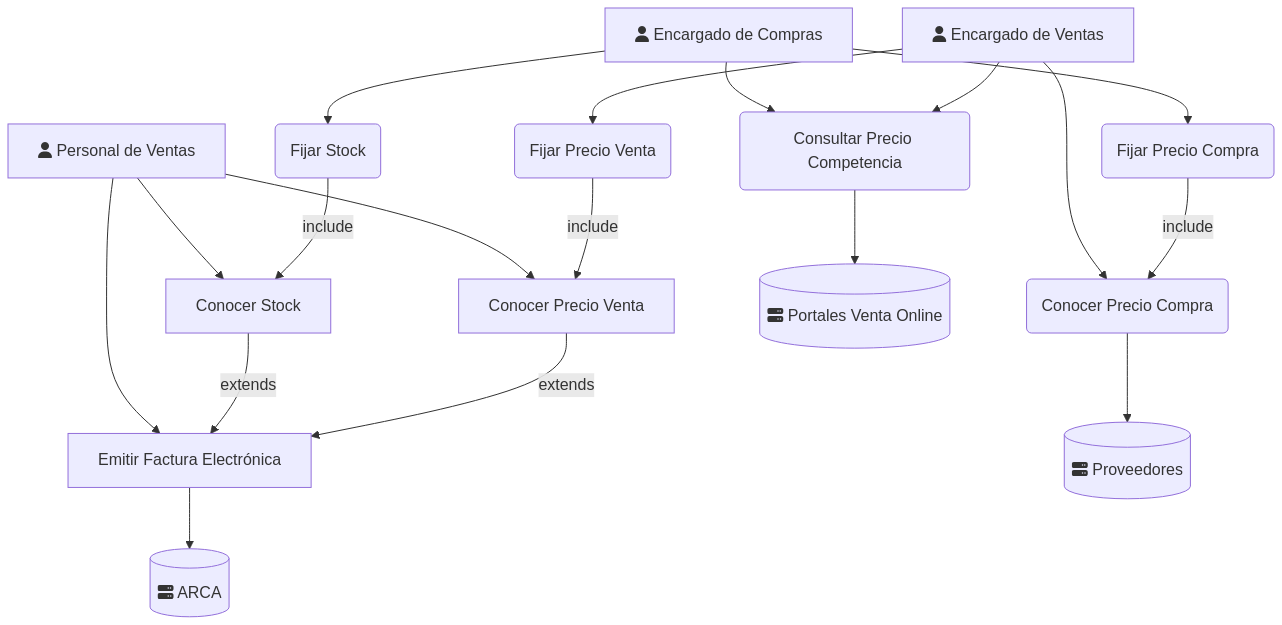
\includegraphics[width=\textwidth]{img/01-diagrama-casos-uso}
	\caption{Diagrama de casos de uso}
	\vspace{15pt}
\end{figure}

\pagebreak

\section{Descripción resumida de casos de uso}

\subsection{Consultar precios disponibles para un producto}

Dado un número de parte (nomenclador único de un producto),
el encargado de compras contará con un listado de precios de dicho producto,
que será descargado de las páginas web e interfaces de programación de los diversos proveedores,
según el caso.

\textbf{Actores:} Encargado de compras (primario), proveedores (secundario).

\subsection{Seguir el stock disponible, previendo necesidades de corto y mediano plazo.}

Dado un ingreso de producto en sucursal,
el encargado de compras debe disponer de un formulario que permita dar de alta el producto en la base de datos propia,
de ser necesario,
y actualizar el stock.

\textbf{Actores:} Encargado de compras (primario).

\subsection{Conocer los precios de recompra}

El encargado de ventas puede necesitar la información del costo de recompra de un producto,
para reaccionar a un cambio en el precio de mercado.
En ocasiones, un precio al cliente final puede caer y el encargado de ventas debe ser capaz de reaccionar a ello.
Este precio se renovará directamente, 
como lo hace cuando el encargado de compras quiere saber qué proveedor ofrece mejores condiciones.

\textbf{Actores:} Encargado de ventas (primario), proveedores (secundario).

\subsection{Conocer los precios de la competencia}

Para poner un precio competitivo,
que cuide a los clientes al tiempo que protege las finanzas de la empresa,
el encargado de ventas debe de disponer del precio de mercado casi en tiempo real.
Para ello, se descargará el mismo, empleando el número de parte,
de portales de venta como ser Mercado Libre y otros.
Con esta información, 
el encargado de ventas definirá los precios de lista de los productos,
que será el precio al consumidor final.

\textbf{Actores:} Encargado de ventas (primario), portales de venta online (secundario).

\subsection{Calcular el margen actual para un producto}

Dado el precio de recompra y el precio de lista establecido por el encargado de compras,
la empresa obtiene un margen por la venta unitaria de los productos.
Sin embargo,
en ocasiones es necesario ofrecer descuentos, disminuyendo dicho margen,
para ofrecer un precio competitivo a clientes institucionales, revendedores u otras empresas.

\textbf{Actores:} Encargado de ventas (primario), proveedores (secundario), portales de venta online (secundario).

\subsection{Consultar precio de un producto}

El personal de venta atiende al comprador minorista y debe consultar el último precio disponible,
decidido ya por el encargado de ventas.
Estos precios pueden cambiar varias veces en una semana y el personal de venta debe estar sincronizado con dichos cambios.

\textbf{Actores:} Personal de ventas (primario), proveedores (secundario).

\subsection{Emitir factura electrónica}

El personal de venta, 
luego de la brindar atención y asesoramiento al comprador minorista,
puede necesitar utilizar la información del sistema
-descripción del producto, cantidad, disponibilidad y precio-
para emitir una factura electrónica.
Esto puede hacerse sincronizando al sistema con la API de la ex AFIP,
ahora ARCA.

\textbf{Actores:} Personal de ventas (primario), Sistema de ARCA (secundario).
